\usetikzlibrary{mindmap,backgrounds}

\begin{center}
\resizebox{0.8\textwidth}{!}{
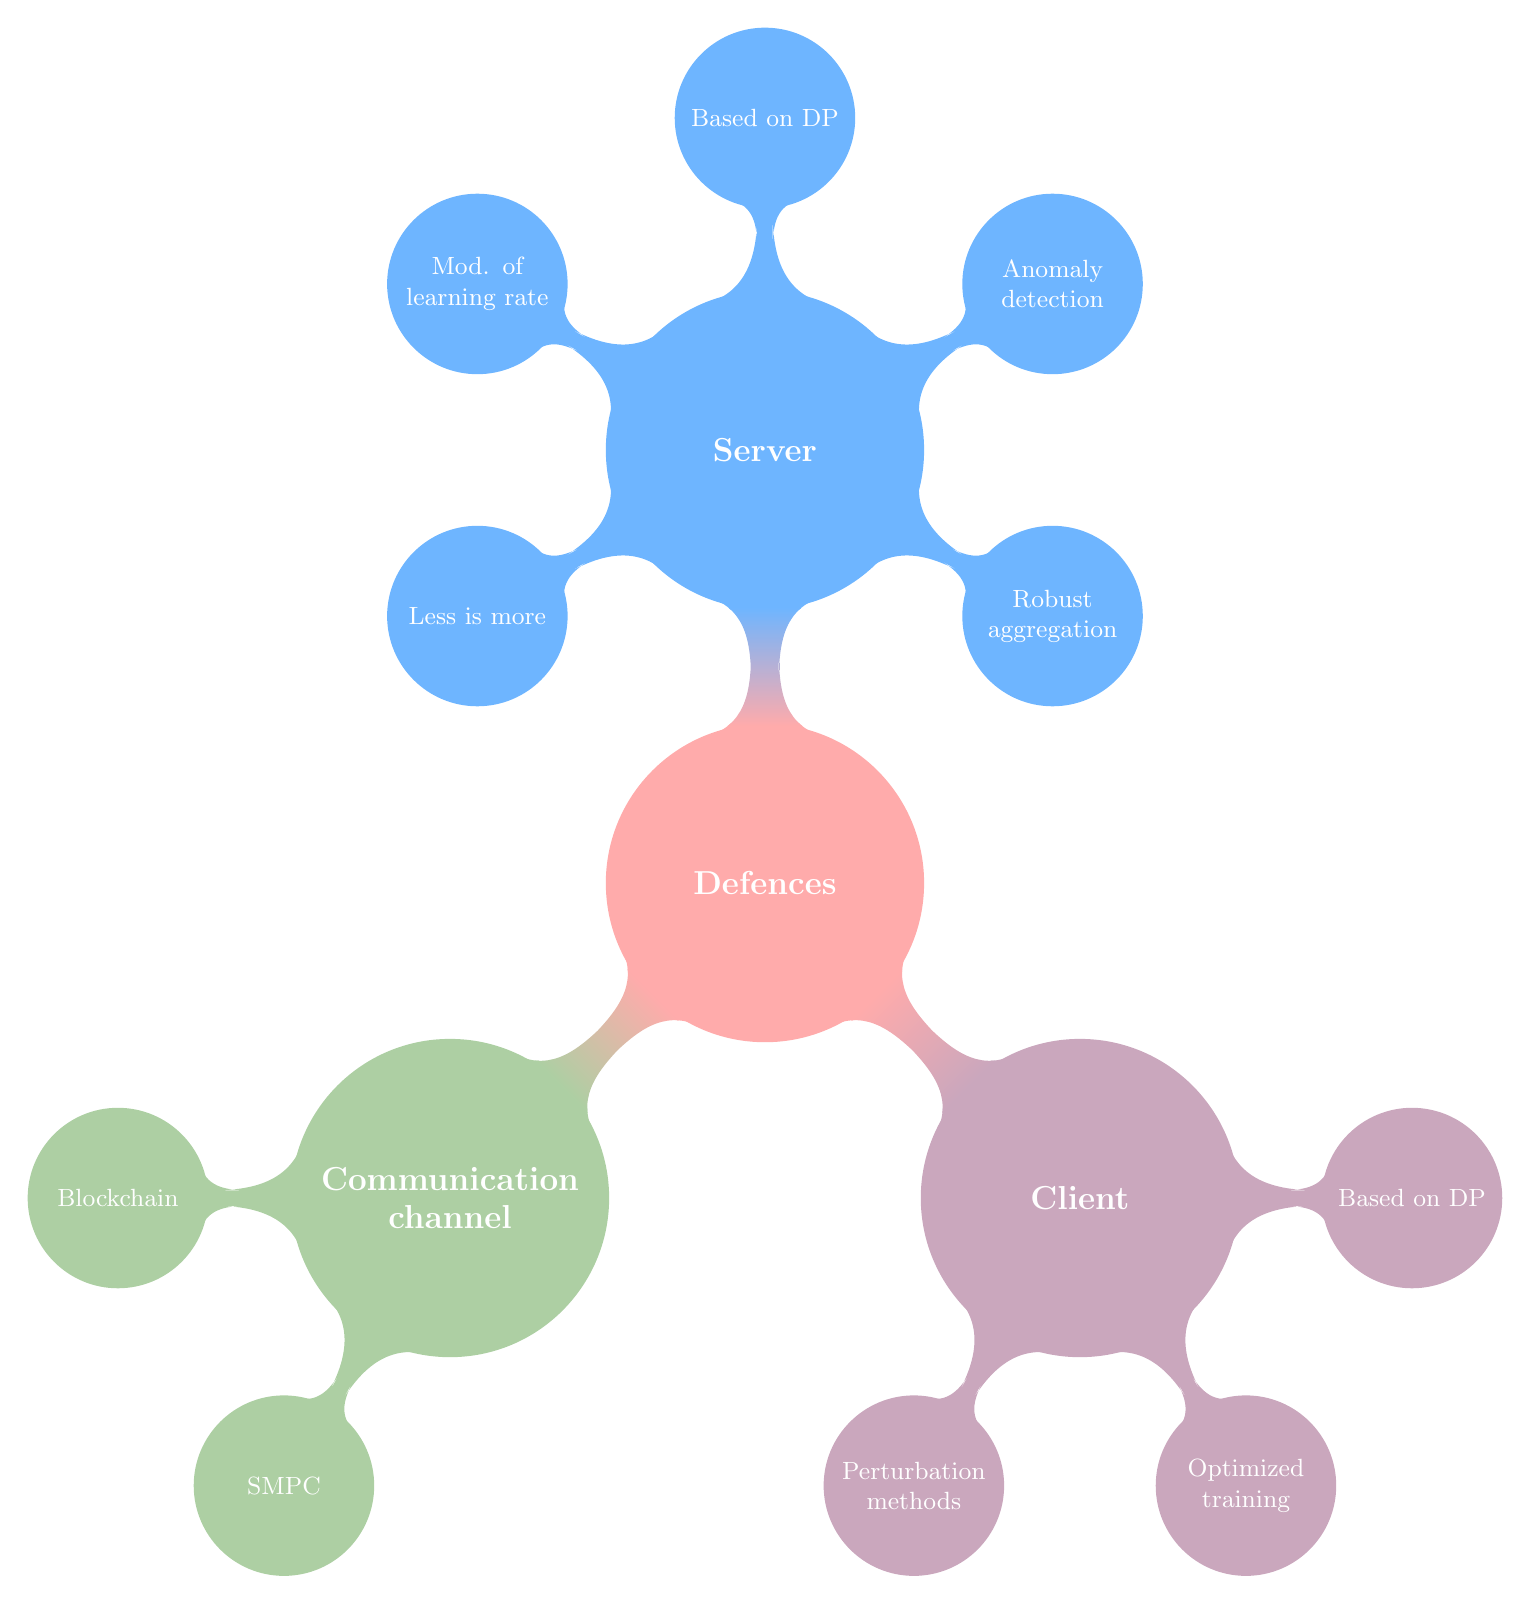
\begin{tikzpicture}[mindmap,
  level 1 concept/.append style={level distance=130,sibling angle=30},
  extra concept/.append style={color=verde_pastel!50,text=black}]

    \definecolor{rojo_pastel}{HTML}{FFABAB}
    \definecolor{azul_pastel}{HTML}{6EB5FF}
    \definecolor{verde_pastel}{HTML}{ADCFA3}
    \definecolor{morado_pastel}{HTML}{CAA7BD}
  % Applied area: computer science and its subfields

  \begin{scope}[mindmap, concept color=rojo_pastel, text=white]
    \node [concept] (def) at (0, 0) {\textbf{Defences}};
  \end{scope}
  
    \begin{scope}[mindmap, concept color=azul_pastel, text=white]
    \node [concept] (ser) at (0, 5.5) {\textbf{Server}}
        child [grow=-30, level distance=120] {node [concept] {Robust aggregation}}
        child [grow=30, level distance=120] {node [concept] {Anomaly detection}}
        child [grow=90, level distance=120] {node [concept] {Based on DP}}
        child [grow=150, level distance=120] {node [concept] {Mod. of learning rate}}
        child [grow=210, level distance=120] {node [concept] {Less is more}};
  \end{scope}
  
    \begin{scope}[mindmap, concept color=verde_pastel, text=white]
    \node [concept] (cli) at (-4, -4) {\textbf{Communication channel}}
        child [grow=180, level distance=120] {node [concept] {Blockchain}
      }
      child [grow=240, level distance=120] {node [concept] {SMPC}};
  \end{scope}
  
    \begin{scope}[mindmap, concept color=morado_pastel, text=white]
    \node [concept] (com) at (4, -4) {\textbf{Client}}
      child [grow=0, level distance=120] {node [concept] {Based on DP}}
      child [grow=-120, level distance=120] {node [concept] {Perturbation methods}}
      child [grow=-60, level distance=120] {node [concept] {Optimized training}};
  \end{scope}
  
    \path (def) to[circle connection bar switch color=from (rojo_pastel) to (azul_pastel)] (ser);
    \path (def) to[circle connection bar switch color=from (rojo_pastel) to (verde_pastel)] (cli);
    \path (def) to[circle connection bar switch color=from (rojo_pastel) to (morado_pastel)] (com);



\end{tikzpicture}}
\end{center}